\chapter{アップグレードに向けたモジュール量産}
前章で述べたように,HL-LHC計画に伴い,内部飛跡検出器のアップグレードが計画されている.本章では,それに伴う,モジュールの量産について説明し,モジュールの構成,要素であるシリコンセンサの原理,フロントエンドASICについて述べ,モジュールの量産について必要な試験項目について説明する.

\section{モジュール量産}
HL-LHC計画にあたって,内部飛跡検出器の総入れ替えを予定しているため,内部に用いるピクセルモジュールの量産が必要である.世界で約10000個のモジュールの量産が計画されており,日本グループはそのうちの約2000個を担当する予定になっている.\\
現在は,実機で用いるモジュールを量産するための準備として,プロトタイプ版のモジュールで量産体制の確認が計画されている.プロトタイプ版のモジュールは2月ごろに完成が予定されている.

\section{ピクセルモジュールの構成}
この節では,ピクセル検出器の構成について説明する.以下にピクセル検出器の構造図を示す.ピクセル検出器はFlex基板,フロントエンドASIC,シリコンピクセルセンサの3要素で構成されている.


\section{シリコンピクセルセンサ}
この節では,ピクセル検出器を構成する要素の1つであるシリコンピクセルセンサについて説明する.

\subsection{シリコンピクセルセンサの原理}
シリコンセンサの動作原理は半導体に従う.この節では,半導体の基本原理と性質について述べる.
物質は導体,絶縁体,半導体の3種に分類することができる.これは,電気抵抗値によって決まっており,半導体は導体と絶縁体の中間の値をもつ.一般に室温で,$10^{-2}$から$10^9 \mathrm{\Omega cm}$の範囲に分類される.典型的な半導体物質にはシリコン,ゲルマニウム,ガリウムヒ素などがあげられる.

\subsubsection*{pn接合と空乏化}
高純度の半導体は,電気を通しにくいが,不純物を添加(ドープ)することによって電気的特性を変えることができる.ホウ素などの3価の元素をドープする場合,これをp型半導体と称する.p型半導体では,価電子帯に電子の欠損である正孔が生じ,これが電気伝導に寄与する.一方ヒ素やリンなど5価の元素をドープする場合は,n型半導体と称する.n型半導体では自由電子が発生し,これが電気伝導に寄与する.p型半導体における不純物をアクセプタ,n型半導体における不純物をドナーと呼ぶ.\\
一般的な半導体検出器は,n型とp型の半導体を接合(pn接合)した構造をもつ.以下の図のよう,n型とp型の接合面付近では,電子-正孔が再結合した空乏層が発生する.これに逆電圧$V_b$を印加することによって空乏層を拡張することができる.このときの電圧$V_b$と空乏層の幅$d$の関係は以下のように求められる.接合面を原点,空乏層を$x_p < x < x_n$とし,ある位置での電位を$V$,電荷密度を$\rho_e$とする.また,各半導体のアクセプタ濃度を$N_a$,ドナー濃度を$N_d$とする.素電荷を$e$,シリコンの誘電率を$\epsilon$とする.

\subsubsection*{荷電粒子の検出}
荷電粒子が物質中の電子との衝突によって失うエネルギーは,Bethe Blochの式であらわされる.

\subsubsection*{エネルギーバンド}
孤立した原子では,エネルギー順位は離散的な値をとる.多数の原子が集めると原子同士の引力と斥力の混じった相互作用により,位置に依存する連続的なバンド状順位をみなすことができる.これをエネルギーバンドという.エネルギーバンド構造は,価電子帯,禁制帯,伝導体から構成される.絶縁体・半導体・導体の違いはこのエネルギーバンド構造の違いによるものである.導体では,バンドが重なっているため,電子やホールといった電荷のキャリアが自由に動くことが可能である.一方で,半導体や絶縁体では,バンド間にギャップがあるため,自由に動くことができない.半導体の場合は,このギャップ幅が$\mathrm{eV}$オーダーであり,熱的な励起によってギャップを超えることが可能になる.絶縁体の場合は,ギャップ幅が約4$\mathrm{eV}$より大きく,室温においてキャリアが自由に動くことができない.

\subsubsection*{ドナーとアクセプタ}


\subsection{バイアス構造}
シリコンピクセルセンサには,製造時に良品不良品を選別するための高電圧用のバイアス構造が備わっている.\\
バンプボンディングの前にセンサのみの試験を行い,動作不良センサを取り除く品質評価の工程がある.このピクセルセンサ評価方法として,IV測定がある.IV測定には全てのピクセルがGNDに落とされている必要があり,また,各ピクセルは分離されている必要がある.そのために必要になるのがバイアス構造である.バイアス構造は,ピクセル間にバイアスレールを置き,そこから各ピクセルにバイアス抵抗を引く.この構造により,ピクセルはGNDと同電位とすることができ,また,各ピクセルが抵抗により,分離される.

\subsection{今回使用したシリコンピクセルセンサ構造}
本論文で扱うピクセルセンサの表面構造について述べる.上から見たセンサの様子である.ピクセルセンサは2次元的に電極が配列されており,センサのみのテストのためにバイアスレールが敷かれている.

\section{HL-LHC ATLAS実験用新型ASIC・RD53A}
この節では,ピクセル検出器からの信号は,検出器に直接接続された電気回路で最初に処理される.この電気回路をフロントエンドエレクトロニクスと呼ぶ.この回路は,全て専用の信号読み出し用ASIC内に実装されている.そのため,フロントエンドASICと呼ぶこともあるが,以降ではASICと呼ぶことにする.\\
この回路を用いて検出器からの微弱な電気信号を受け取り,計測用のシステムに最適化した応答をするように信号をアンプ回路や波形整形回路などで調整する.さらに,コンピュータでの解析処理や,データの保存のためにアナログ信号をデジタル信号に変換する.\\
以下にピクセル検出器と読み出しASICの接続図を示す.ピクセル検出器の各チャンネルとASICはバンプボンディングという手法で接合し,ASICでは検出器からの信号に対して処理を行う.\\


RD53AはHL-LHC ATLAS実験用に開発されたプロトタイプ版の新型ASICであり,前章で述べたような,高い放射線耐性と,高い位置分解能を達成する.以下に現行のATLAS検出器で用いられているASIC・FEI4とFEI3,プロトタイプ版新型ASIC・RD53Aの比較を示す.

\begin{table}[h]
  \centering
  \caption{現行のASIC2種と新型プロトタイプ版ASICの比較}
  \begin{tabular} {|l|cc|c|} \hline
    ASIC名 & FEI3 & FEI4 & RD53A \\ \hline \hline
    ピクセルサイズ & 50 $\times$ 400 $\mathrm{\mu m^2}$ & 50 $\times$ 250 $\mathrm{\mu m^2}$ & 50 $\times$ 50 $\mathrm{\mu m^2}$ \\
    ピクセルのチャンネル数 & 18 $\times$ 160 & 80 $\times$ 336 & 50 $\times$ 50 $\mathrm{\mu m^2}$ \\ 
    チップサイズ & 7.6 $\times$ 10.8 $\mathrm{mm^2}$ & 20.2 $\times$ 19.0 $\mathrm{mm^2}$ & 20 $\times$ 11.8 $\mathrm{mm^2}$\\ \hline
  \end{tabular}
  \label{tab:ASIC}
\end{table}

このように,RD53Aは現行のASICと比較してピクセルサイズが小さいため,高い位置分解能を達成する.

\subsection{レジスタ}
ASICには,アナログ回路とデジタル回路の振る舞いを調節するために,回路の動作を制御する設定値を保持するレジスタが存在する.RD53Aのレジスタは2種類存在し,全てのピクセルに共通の設定を保存するグローバルレジスタ(GR)と各ピクセルの設定値を保持するピクセルレジスタ(PR)がある.
\begin{itemize}
\item グローバルレジスタ\\
  RD53Aには137個のGRがあり,ピクセルに共通が閾値(threshold),回路のオンオフなどを設定することができる.
\item ピクセルレジスタ\\
  Synchronus Frontendには3 $\mathrm{bit}$,その他の2つのフロントエンドには8 $\mathrm{bit}$のレジスタがある.ピクセルのデジタル回路のオンオフや閾値(threshold)を設定することができる.
\end{itemize}


\subsection{RD53Aフロントエンドデザイン}
RD53Aはプロトタイプ版のため,Synchronase Frontend, Linear Frontend, Differential Frontendと,3つの異なるフロントエンドデザインが存在する.

\begin{figure}[h]
\centering
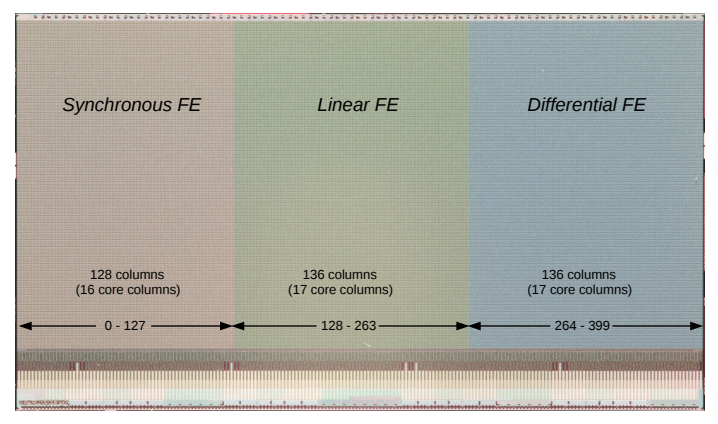
\includegraphics[width=8cm]{./figure/RD53A_FE.png}
\caption{RD53Aのフロントエンドデザイン}
\label{fig:RD53AFE}
\end{figure}

今回は実機で利用されることが予定されているDifferential Frontend(以下:Diff FE)のみを用いて研究を行なったため,それについて詳しく説明する.

\subsubsection*{Diff FEの仕組み}
3つのフロントエンドで大きく異なるのは,アナログ回路部分の構造である.Diff FEのアナログ回路構造を以下に示す.\\

\begin{figure}[h]
\centering
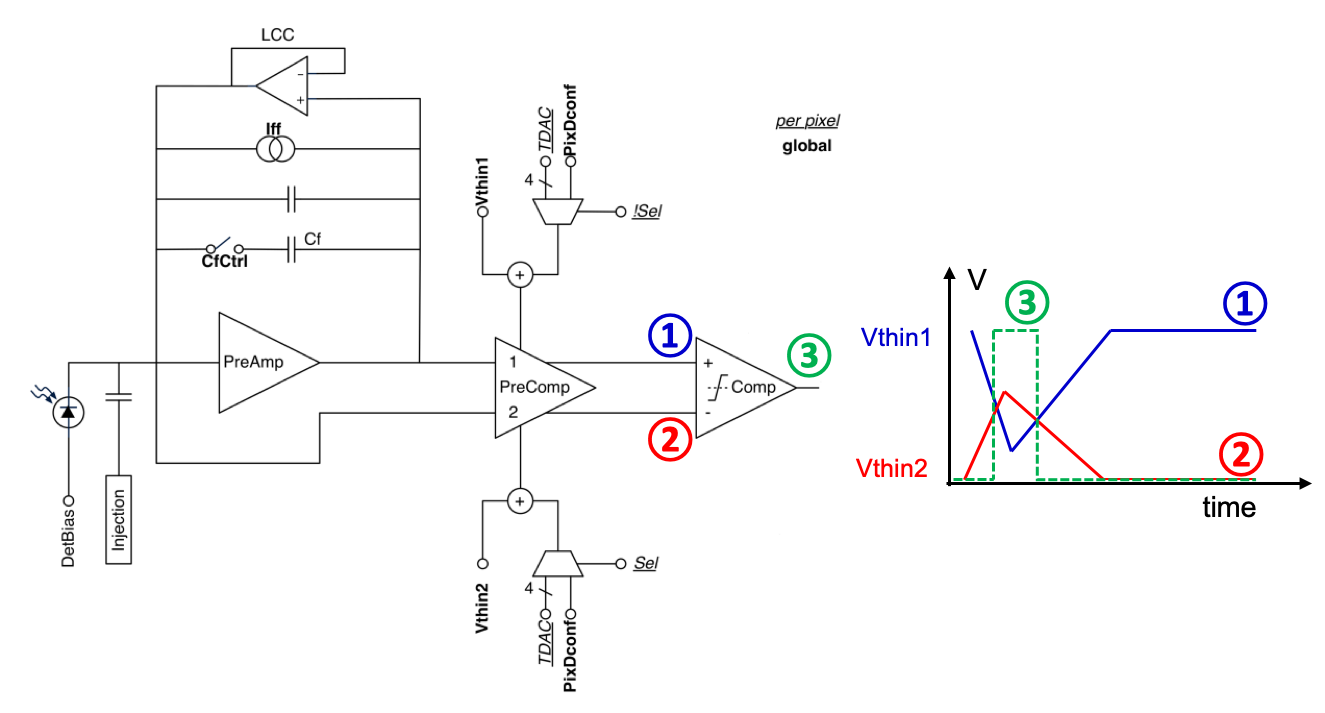
\includegraphics[width=8cm]{./figure/RD53A_DiffFE.png}
\caption{Diff FEのアナログ回路構造}
\label{fig:DiffFE}
\end{figure}

図\ref{fig:DiffFE}に示したように,Diff FEでは,RD53AのGR値である''DiffVthin1''と''DiffVthin2''で閾値を設定可能である.これらのGR値は,入力された信号(\ref{fig:DiffFE}の赤い信号)と,それに対して反転増幅を行なった後の信号(\ref{fig:DiffFE}の青い信号)それぞれに作用するオフセット電圧である.Diff FEはこれらの信号の差動によって,出力信号を定義しているため,オフセットを変化させることで,閾値を調整することができる.

\subsection{RD53Aのデータ収集の仕組み}
図\ref{fig:RD53Aprc}にRD53Aのデータ収集の仕組みを示す.まず,Hitとされる信号(センサからの信号はBinary in from FEから,擬似パルスによる信号はCAL_edgeから)が入射する.各ピクセルごとに設定されている''Enable''がオンの場合,そのピクセルのデータは
と''HirOr Enable''が共にオンの場合,

\begin{figure}[h]
  \centering
  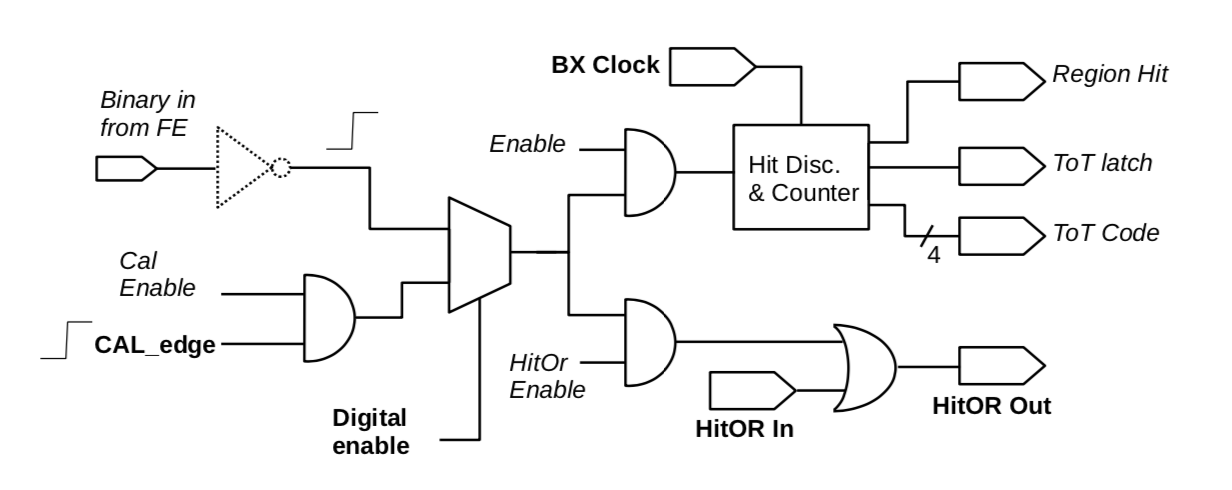
\includegraphics[width=8cm]{./figure/RD53Aproc.png}
  \caption{RD53Aのデータ収集の仕組み.全ピクセルに共通する信号が太字,ピクセルごとに記録されている信号が斜体文字になっている.}
  \label{fig:RD53Aproc}
\end{figure}




\subsection{HitOR信号}
RD53Aには,現行のFEI4に実装されているセルフトリガ機能がない代わりに,HitORというセンサに荷電粒子が入射したタイミングで,出力される信号が存在する.HitOR信号出力する仕組みについて説明する.図\ref{fig:HitOR}はRD53Aの一部である$8 \times 8 \mathrm{pixel}$を示している.

\begin{figure}[h]
\centering
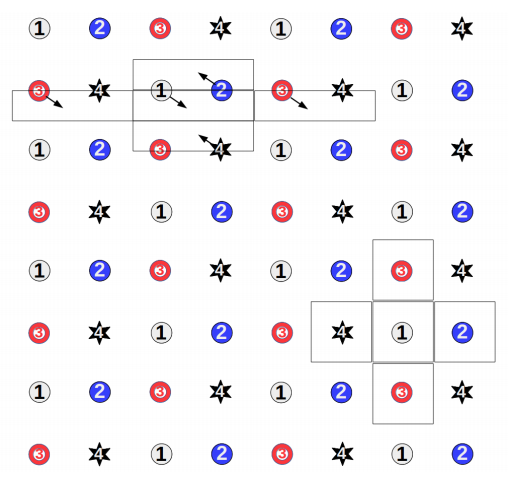
\includegraphics[width=8cm]{./figure/HitOR.png}
\caption{HitOR信号のネットワーク図}
\label{fig:HitOR}
\end{figure}

HitOR信号は,図\ref{HitOR}の各ピクセルに割り当てられている番号1-4ごとにまとめて読み出される.これを番号ごとにネットワークと呼ぶ.このネットワークは任意のネットワークに含まれるピクセルの上下に1つのネットワーク,左右に異なる2つのネットワークが存在するように配置されている.例えば,1番のネットワークのあるピクセルには,3番のネットワークが上下に存在し,左右には2番と4番のネットワークが存在するようになっている.このように配置されたネットワークごとに,HitORは読み出される仕組みになっている.

\section{モジュール量産に向けた品質性能試験}
量産されたモジュールは品質性能基準を達成するために,試験にかけられる.その試験項目の1つとして,本論文に関わる,粒子線に対する応答評価試験が存在する.

\subsection{粒子線に対する応答評価試験の意義}
HL-LHC ATLAS実験に向けたピクセル検出器量産に際して,全ての検出器モジュールに対して,品質管理のための試験を行う.この試験項目の1つとして,粒子線に対する応答評価試験(以下:ソーススキャン)が設けられている.\\
前章でも述べたように,ピクセル検出器の各チャンネルとASICはバンプボンディングという手法で接続されている.このバンプボンディングに異常がないかどうかを確認するための試験が,ソーススキャンである.\\

\subsection{応答評価試験の手法}
応答評価試験には,主に2種類の手法がある.1つは,センサに荷電粒子が入射した時の信号を取得したタイミングでデータ取得を行う,セルフトリガと呼ばれる手法.もう1つは,センサの上にシンチレータ,その上に粒子線源を設置し,シンチレータに粒子線が入射した時の信号を取得したタイミングでデータ取得を行う手法である.今回はこれら2種類の手法を用いてソーススキャンを行い,どのような試験結果の振る舞いがなされるかの検証を行なった.\\
今回用いた読み出しASIC・RD53Aには,セルフトリガ機能が実装されていないため,HitOR信号を外部に出力し,FPGAを用いて処理することでデータ取得を行なった.\\
YARRソフトウェアには,外部トリガスキャンという機能が実装されているため,今回はこの外部トリガにHitOR信号を用いた手法をセルフトリガ,シンチレータに粒子線が入射した時の信号を用いた手法を外部トリガと呼ぶ.

\subsection{本研究の目的}
本研究では,シリコンピクセルセンサが接続されたHL-LHC ATLAS実験用新型ASIC搭載モジュールを用いて,2種類の手法で行なったの粒子線に対する応答評価試験結果について報告する.
